\documentclass[1p]{elsarticle_modified}
%\bibliographystyle{elsarticle-num}

%\usepackage[colorlinks]{hyperref}
%\usepackage{abbrmath_seonhwa} %\Abb, \Ascr, \Acal ,\Abf, \Afrak
\usepackage{amsfonts}
\usepackage{amssymb}
\usepackage{amsmath}
\usepackage{amsthm}
\usepackage{scalefnt}
\usepackage{amsbsy}
\usepackage{kotex}
\usepackage{caption}
\usepackage{subfig}
\usepackage{color}
\usepackage{graphicx}
\usepackage{xcolor} %% white, black, red, green, blue, cyan, magenta, yellow
\usepackage{float}
\usepackage{setspace}
\usepackage{hyperref}

\usepackage{tikz}
\usetikzlibrary{arrows}

\usepackage{multirow}
\usepackage{array} % fixed length table
\usepackage{hhline}

%%%%%%%%%%%%%%%%%%%%%
\makeatletter
\renewcommand*\env@matrix[1][\arraystretch]{%
	\edef\arraystretch{#1}%
	\hskip -\arraycolsep
	\let\@ifnextchar\new@ifnextchar
	\array{*\c@MaxMatrixCols c}}
\makeatother %https://tex.stackexchange.com/questions/14071/how-can-i-increase-the-line-spacing-in-a-matrix
%%%%%%%%%%%%%%%

\usepackage[normalem]{ulem}

\newcommand{\msout}[1]{\ifmmode\text{\sout{\ensuremath{#1}}}\else\sout{#1}\fi}
%SOURCE: \msout is \stkout macro in https://tex.stackexchange.com/questions/20609/strikeout-in-math-mode

\newcommand{\cancel}[1]{
	\ifmmode
	{\color{red}\msout{#1}}
	\else
	{\color{red}\sout{#1}}
	\fi
}

\newcommand{\add}[1]{
	{\color{blue}\uwave{#1}}
}

\newcommand{\replace}[2]{
	\ifmmode
	{\color{red}\msout{#1}}{\color{blue}\uwave{#2}}
	\else
	{\color{red}\sout{#1}}{\color{blue}\uwave{#2}}
	\fi
}

\newcommand{\Sol}{\mathcal{S}} %segment
\newcommand{\D}{D} %diagram
\newcommand{\A}{\mathcal{A}} %arc


%%%%%%%%%%%%%%%%%%%%%%%%%%%%%5 test

\def\sl{\operatorname{\textup{SL}}(2,\Cbb)}
\def\psl{\operatorname{\textup{PSL}}(2,\Cbb)}
\def\quan{\mkern 1mu \triangleright \mkern 1mu}

\theoremstyle{definition}
\newtheorem{thm}{Theorem}[section]
\newtheorem{prop}[thm]{Proposition}
\newtheorem{lem}[thm]{Lemma}
\newtheorem{ques}[thm]{Question}
\newtheorem{cor}[thm]{Corollary}
\newtheorem{defn}[thm]{Definition}
\newtheorem{exam}[thm]{Example}
\newtheorem{rmk}[thm]{Remark}
\newtheorem{alg}[thm]{Algorithm}

\newcommand{\I}{\sqrt{-1}}
\begin{document}

%\begin{frontmatter}
%
%\title{Boundary parabolic representations of knots up to 8 crossings}
%
%%% Group authors per affiliation:
%\author{Yunhi Cho} 
%\address{Department of Mathematics, University of Seoul, Seoul, Korea}
%\ead{yhcho@uos.ac.kr}
%
%
%\author{Seonhwa Kim} %\fnref{s_kim}}
%\address{Center for Geometry and Physics, Institute for Basic Science, Pohang, 37673, Korea}
%\ead{ryeona17@ibs.re.kr}
%
%\author{Hyuk Kim}
%\address{Department of Mathematical Sciences, Seoul National University, Seoul 08826, Korea}
%\ead{hyukkim@snu.ac.kr}
%
%\author{Seokbeom Yoon}
%\address{Department of Mathematical Sciences, Seoul National University, Seoul, 08826,  Korea}
%\ead{sbyoon15@snu.ac.kr}
%
%\begin{abstract}
%We find all boundary parabolic representation of knots up to 8 crossings.
%
%\end{abstract}
%\begin{keyword}
%    \MSC[2010] 57M25 
%\end{keyword}
%
%\end{frontmatter}

%\linenumbers
%\tableofcontents
%
\newcommand\colored[1]{\textcolor{white}{\rule[-0.35ex]{0.8em}{1.4ex}}\kern-0.8em\color{red} #1}%
%\newcommand\colored[1]{\textcolor{white}{ #1}\kern-2.17ex	\textcolor{white}{ #1}\kern-1.81ex	\textcolor{white}{ #1}\kern-2.15ex\color{red}#1	}

{\Large $\underline{11n_{157}~(K11n_{157})}$}

\setlength{\tabcolsep}{10pt}
\renewcommand{\arraystretch}{1.6}
\vspace{1cm}\begin{tabular}{m{100pt}>{\centering\arraybackslash}m{274pt}}
\multirow{5}{120pt}{
	\centering
	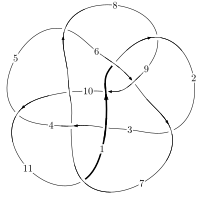
\includegraphics[width=112pt]{../../../GIT/diagram.site/Diagrams/png/773_11n_157.png}\\
\ \ \ A knot diagram\footnotemark}&
\allowdisplaybreaks
\textbf{Linearized knot diagam} \\
\cline{2-2}
 &
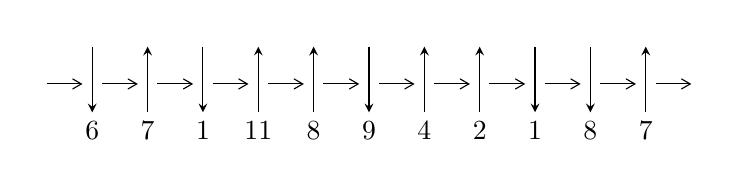
\begin{tikzpicture}[x=20pt, y=17pt]
	% nodes
	\node (C0) at (0, 0) {};
	\node (C1) at (1, 0) {};
	\node (C1U) at (1, +1) {};
	\node (C1D) at (1, -1) {6};

	\node (C2) at (2, 0) {};
	\node (C2U) at (2, +1) {};
	\node (C2D) at (2, -1) {7};

	\node (C3) at (3, 0) {};
	\node (C3U) at (3, +1) {};
	\node (C3D) at (3, -1) {1};

	\node (C4) at (4, 0) {};
	\node (C4U) at (4, +1) {};
	\node (C4D) at (4, -1) {11};

	\node (C5) at (5, 0) {};
	\node (C5U) at (5, +1) {};
	\node (C5D) at (5, -1) {8};

	\node (C6) at (6, 0) {};
	\node (C6U) at (6, +1) {};
	\node (C6D) at (6, -1) {9};

	\node (C7) at (7, 0) {};
	\node (C7U) at (7, +1) {};
	\node (C7D) at (7, -1) {4};

	\node (C8) at (8, 0) {};
	\node (C8U) at (8, +1) {};
	\node (C8D) at (8, -1) {2};

	\node (C9) at (9, 0) {};
	\node (C9U) at (9, +1) {};
	\node (C9D) at (9, -1) {1};

	\node (C10) at (10, 0) {};
	\node (C10U) at (10, +1) {};
	\node (C10D) at (10, -1) {8};

	\node (C11) at (11, 0) {};
	\node (C11U) at (11, +1) {};
	\node (C11D) at (11, -1) {7};
	\node (C12) at (12, 0) {};

	% arrows
	\draw[->,>={angle 60}]
	(C0) edge (C1) (C1) edge (C2) (C2) edge (C3) (C3) edge (C4) (C4) edge (C5) (C5) edge (C6) (C6) edge (C7) (C7) edge (C8) (C8) edge (C9) (C9) edge (C10) (C10) edge (C11) (C11) edge (C12) ;	\draw[->,>=stealth]
	(C1U) edge (C1D) (C2D) edge (C2U) (C3U) edge (C3D) (C4D) edge (C4U) (C5D) edge (C5U) (C6U) edge (C6D) (C7D) edge (C7U) (C8D) edge (C8U) (C9U) edge (C9D) (C10U) edge (C10D) (C11D) edge (C11U) ;
	\end{tikzpicture} \\
\hhline{~~} \\& 
\textbf{Solving Sequence} \\ \cline{2-2} 
 &
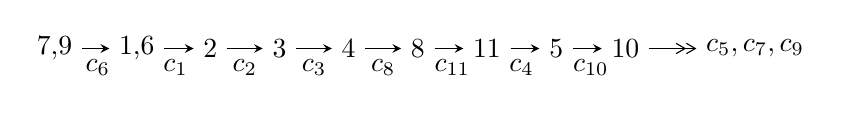
\begin{tikzpicture}[x=25pt, y=7pt]
	% node
	\node (A0) at (-1/8, 0) {7,9};
	\node (A1) at (17/16, 0) {1,6};
	\node (A2) at (17/8, 0) {2};
	\node (A3) at (25/8, 0) {3};
	\node (A4) at (33/8, 0) {4};
	\node (A5) at (41/8, 0) {8};
	\node (A6) at (49/8, 0) {11};
	\node (A7) at (57/8, 0) {5};
	\node (A8) at (65/8, 0) {10};
	\node (C1) at (1/2, -1) {$c_{6}$};
	\node (C2) at (13/8, -1) {$c_{1}$};
	\node (C3) at (21/8, -1) {$c_{2}$};
	\node (C4) at (29/8, -1) {$c_{3}$};
	\node (C5) at (37/8, -1) {$c_{8}$};
	\node (C6) at (45/8, -1) {$c_{11}$};
	\node (C7) at (53/8, -1) {$c_{4}$};
	\node (C8) at (61/8, -1) {$c_{10}$};
	\node (A9) at (10, 0) {$c_{5},c_{7},c_{9}$};

	% edge
	\draw[->,>=stealth]	
	(A0) edge (A1) (A1) edge (A2) (A2) edge (A3) (A3) edge (A4) (A4) edge (A5) (A5) edge (A6) (A6) edge (A7) (A7) edge (A8) ;
	\draw[->>,>={angle 60}]	
	(A8) edge (A9);
\end{tikzpicture} \\ 

\end{tabular} \\

\footnotetext{
The image of knot diagram is generated by the software ``\textbf{Draw programme}" developed by Andrew Bartholomew(\url{http://www.layer8.co.uk/maths/draw/index.htm\#Running-draw}), where we modified some parts for our purpose(\url{https://github.com/CATsTAILs/LinksPainter}).
}\phantom \\ \newline 
\centering \textbf{Ideals for irreducible components\footnotemark of $X_{\text{par}}$} 
 
\begin{align*}
I^u_{1}&=\langle 
6371 u^{14}+7974 u^{13}+\cdots+2417 b+9214,\;-7643 u^{14}-6072 u^{13}+\cdots+2417 a-4421,\\
\phantom{I^u_{1}}&\phantom{= \langle  }u^{15}+2 u^{14}+u^{13}- u^{12}+5 u^{11}+12 u^{10}+11 u^9+5 u^8+8 u^7+14 u^6+11 u^5+5 u^4+2 u^3+3 u^2+3 u+1\rangle \\
I^u_{2}&=\langle 
-8.78150\times10^{28} u^{27}+5.66569\times10^{28} u^{26}+\cdots+6.30688\times10^{29} b-6.14221\times10^{29},\\
\phantom{I^u_{2}}&\phantom{= \langle  }3.22564\times10^{28} u^{27}-1.12906\times10^{28} u^{26}+\cdots+3.94180\times10^{28} a+5.37899\times10^{29},\;u^{28}-3 u^{26}+\cdots+15 u+7\rangle \\
I^u_{3}&=\langle 
u^8-2 u^7- u^6+3 u^5+2 u^4-6 u^3-4 u^2+3 b+5 u,\;2 u^8-2 u^7-3 u^6+4 u^5+7 u^4-5 u^3-8 u^2+3 a+8 u+4,\\
\phantom{I^u_{3}}&\phantom{= \langle  }u^9- u^8- u^7+u^6+3 u^5- u^4-3 u^3+u^2+1\rangle \\
I^u_{4}&=\langle 
- u^3-2 u^2+2 b-4 u-1,\;a,\;u^4+u^3+2 u^2- u+1\rangle \\
I^u_{5}&=\langle 
b- u,\;a,\;u^2- u+1\rangle \\
\\
\end{align*}
\raggedright * 5 irreducible components of $\dim_{\mathbb{C}}=0$, with total 58 representations.\\
\footnotetext{All coefficients of polynomials are rational numbers. But the coefficients are sometimes approximated in decimal forms when there is not enough margin.}
\newpage
\renewcommand{\arraystretch}{1}
\centering \section*{I. $I^u_{1}= \langle 6371 u^{14}+7974 u^{13}+\cdots+2417 b+9214,\;-7643 u^{14}-6072 u^{13}+\cdots+2417 a-4421,\;u^{15}+2 u^{14}+\cdots+3 u+1 \rangle$}
\flushleft \textbf{(i) Arc colorings}\\
\begin{tabular}{m{7pt} m{180pt} m{7pt} m{180pt} }
\flushright $a_{7}=$&$\begin{pmatrix}1\\0\end{pmatrix}$ \\
\flushright $a_{9}=$&$\begin{pmatrix}0\\u\end{pmatrix}$ \\
\flushright $a_{1}=$&$\begin{pmatrix}3.16218 u^{14}+2.51221 u^{13}+\cdots+8.43235 u+1.82913\\-2.63591 u^{14}-3.29913 u^{13}+\cdots-7.27431 u-3.81216\end{pmatrix}$ \\
\flushright $a_{6}=$&$\begin{pmatrix}1\\- u^2\end{pmatrix}$ \\
\flushright $a_{2}=$&$\begin{pmatrix}3.16218 u^{14}+2.51221 u^{13}+\cdots+7.43235 u+1.82913\\-2.63591 u^{14}-3.29913 u^{13}+\cdots-7.27431 u-3.81216\end{pmatrix}$ \\
\flushright $a_{3}=$&$\begin{pmatrix}0.526272 u^{14}-0.786926 u^{13}+\cdots+0.158047 u-1.98304\\-2.63591 u^{14}-3.29913 u^{13}+\cdots-7.27431 u-3.81216\end{pmatrix}$ \\
\flushright $a_{4}=$&$\begin{pmatrix}-2.88829 u^{14}-1.53496 u^{13}+\cdots-10.3910 u-1.51055\\2.07654 u^{14}+3.02234 u^{13}+\cdots+6.23211 u+2.68722\end{pmatrix}$ \\
\flushright $a_{8}=$&$\begin{pmatrix}-14.2950 u^{14}-17.2429 u^{13}+\cdots-37.4675 u-19.5999\\3.86512 u^{14}+5.89036 u^{13}+\cdots+12.4721 u+7.53496\end{pmatrix}$ \\
\flushright $a_{11}=$&$\begin{pmatrix}5.79810 u^{14}+5.81134 u^{13}+\cdots+15.7067 u+5.64129\\-2.63591 u^{14}-3.29913 u^{13}+\cdots-7.27431 u-3.81216\end{pmatrix}$ \\
\flushright $a_{5}=$&$\begin{pmatrix}9.56144 u^{14}+16.6558 u^{13}+\cdots+17.5350 u+18.8192\\1.10716 u^{14}+1.23128 u^{13}+\cdots+2.12495 u-1.23790\end{pmatrix}$ \\
\flushright $a_{10}=$&$\begin{pmatrix}-19.5668 u^{14}-23.8411 u^{13}+\cdots-54.0161 u-27.2242\\6.56103 u^{14}+10.1800 u^{13}+\cdots+19.0364 u+11.4803\end{pmatrix}$\\ \flushright $a_{10}=$&$\begin{pmatrix}-19.5668 u^{14}-23.8411 u^{13}+\cdots-54.0161 u-27.2242\\6.56103 u^{14}+10.1800 u^{13}+\cdots+19.0364 u+11.4803\end{pmatrix}$\\&\end{tabular}
\flushleft \textbf{(ii) Obstruction class $= -1$}\\~\\
\flushleft \textbf{(iii) Cusp Shapes $= -\frac{1121}{2417} u^{14}-\frac{15391}{2417} u^{13}+\cdots+\frac{7549}{2417} u-\frac{21392}{2417}$}\\~\\
\newpage\renewcommand{\arraystretch}{1}
\flushleft \textbf{(iv) u-Polynomials at the component}\newline \\
\begin{tabular}{m{50pt}|m{274pt}}
Crossings & \hspace{64pt}u-Polynomials at each crossing \\
\hline $$\begin{aligned}c_{1},c_{6}\end{aligned}$$&$\begin{aligned}
&u^{15}-2 u^{14}+\cdots+3 u-1
\end{aligned}$\\
\hline $$\begin{aligned}c_{2},c_{5}\end{aligned}$$&$\begin{aligned}
&u^{15}+4 u^{13}+\cdots+21 u-7
\end{aligned}$\\
\hline $$\begin{aligned}c_{3},c_{10}\end{aligned}$$&$\begin{aligned}
&u^{15}- u^{14}+\cdots+9 u+1
\end{aligned}$\\
\hline $$\begin{aligned}c_{4},c_{11}\end{aligned}$$&$\begin{aligned}
&u^{15}- u^{14}+\cdots+3 u-1
\end{aligned}$\\
\hline $$\begin{aligned}c_{7}\end{aligned}$$&$\begin{aligned}
&u^{15}-9 u^{14}+\cdots+89 u-13
\end{aligned}$\\
\hline $$\begin{aligned}c_{8}\end{aligned}$$&$\begin{aligned}
&u^{15}-16 u^{14}+\cdots-384 u+64
\end{aligned}$\\
\hline $$\begin{aligned}c_{9}\end{aligned}$$&$\begin{aligned}
&u^{15}-18 u^{14}+\cdots+166 u-13
\end{aligned}$\\
\hline
\end{tabular}\\~\\
\newpage\renewcommand{\arraystretch}{1}
\flushleft \textbf{(v) Riley Polynomials at the component}\newline \\
\begin{tabular}{m{50pt}|m{274pt}}
Crossings & \hspace{64pt}Riley Polynomials at each crossing \\
\hline $$\begin{aligned}c_{1},c_{6}\end{aligned}$$&$\begin{aligned}
&y^{15}-2 y^{14}+\cdots+3 y-1
\end{aligned}$\\
\hline $$\begin{aligned}c_{2},c_{5}\end{aligned}$$&$\begin{aligned}
&y^{15}+8 y^{14}+\cdots-371 y-49
\end{aligned}$\\
\hline $$\begin{aligned}c_{3},c_{10}\end{aligned}$$&$\begin{aligned}
&y^{15}-23 y^{14}+\cdots+143 y-1
\end{aligned}$\\
\hline $$\begin{aligned}c_{4},c_{11}\end{aligned}$$&$\begin{aligned}
&y^{15}+17 y^{14}+\cdots-9 y-1
\end{aligned}$\\
\hline $$\begin{aligned}c_{7}\end{aligned}$$&$\begin{aligned}
&y^{15}-3 y^{14}+\cdots-633 y-169
\end{aligned}$\\
\hline $$\begin{aligned}c_{8}\end{aligned}$$&$\begin{aligned}
&y^{15}-6 y^{14}+\cdots+49152 y-4096
\end{aligned}$\\
\hline $$\begin{aligned}c_{9}\end{aligned}$$&$\begin{aligned}
&y^{15}-14 y^{14}+\cdots+1972 y-169
\end{aligned}$\\
\hline
\end{tabular}\\~\\
\newpage\flushleft \textbf{(vi) Complex Volumes and Cusp Shapes}
$$\begin{array}{c|c|c}  
\text{Solutions to }I^u_{1}& \I (\text{vol} + \sqrt{-1}CS) & \text{Cusp shape}\\
 \hline 
\begin{aligned}
u &= \phantom{-}0.612704 + 0.756856 I \\
a &= \phantom{-}0.341418 - 0.122016 I \\
b &= \phantom{-}0.566944 + 0.416117 I\end{aligned}
 & \phantom{-}0.01045 - 1.91554 I & \phantom{-}0.97885 + 4.27627 I \\ \hline\begin{aligned}
u &= \phantom{-}0.612704 - 0.756856 I \\
a &= \phantom{-}0.341418 + 0.122016 I \\
b &= \phantom{-}0.566944 - 0.416117 I\end{aligned}
 & \phantom{-}0.01045 + 1.91554 I & \phantom{-}0.97885 - 4.27627 I \\ \hline\begin{aligned}
u &= -0.749863 + 0.844909 I \\
a &= -0.867808 - 0.597101 I \\
b &= -0.124797 - 0.345224 I\end{aligned}
 & \phantom{-}3.80312 + 4.84275 I & \phantom{-}6.83327 - 2.97437 I \\ \hline\begin{aligned}
u &= -0.749863 - 0.844909 I \\
a &= -0.867808 + 0.597101 I \\
b &= -0.124797 + 0.345224 I\end{aligned}
 & \phantom{-}3.80312 - 4.84275 I & \phantom{-}6.83327 + 2.97437 I \\ \hline\begin{aligned}
u &= -0.864919\phantom{ +0.000000I} \\
a &= -0.417102\phantom{ +0.000000I} \\
b &= -0.552891\phantom{ +0.000000I}\end{aligned}
 & \phantom{-}1.96166\phantom{ +0.000000I} & \phantom{-}8.66210\phantom{ +0.000000I} \\ \hline\begin{aligned}
u &= -0.330359 + 0.744277 I \\
a &= -0.712671 + 0.196118 I \\
b &= -0.743805 + 0.481051 I\end{aligned}
 & \phantom{-}1.29784 - 0.91531 I & \phantom{-}6.30482 + 3.51826 I \\ \hline\begin{aligned}
u &= -0.330359 - 0.744277 I \\
a &= -0.712671 - 0.196118 I \\
b &= -0.743805 - 0.481051 I\end{aligned}
 & \phantom{-}1.29784 + 0.91531 I & \phantom{-}6.30482 - 3.51826 I \\ \hline\begin{aligned}
u &= \phantom{-}0.551581 + 0.527918 I \\
a &= \phantom{-}3.41165 - 0.50064 I \\
b &= \phantom{-}0.17287 - 1.44617 I\end{aligned}
 & -7.32770 - 5.27705 I & -2.66781 + 10.56442 I \\ \hline\begin{aligned}
u &= \phantom{-}0.551581 - 0.527918 I \\
a &= \phantom{-}3.41165 + 0.50064 I \\
b &= \phantom{-}0.17287 + 1.44617 I\end{aligned}
 & -7.32770 + 5.27705 I & -2.66781 - 10.56442 I \\ \hline\begin{aligned}
u &= -0.620336 + 0.202077 I \\
a &= -3.98780 + 1.70604 I \\
b &= \phantom{-}0.32367 - 1.38455 I\end{aligned}
 & -8.37106 - 3.72407 I & -11.66592 - 1.71457 I\\
 \hline 
 \end{array}$$\newpage$$\begin{array}{c|c|c}  
\text{Solutions to }I^u_{1}& \I (\text{vol} + \sqrt{-1}CS) & \text{Cusp shape}\\
 \hline 
\begin{aligned}
u &= -0.620336 - 0.202077 I \\
a &= -3.98780 - 1.70604 I \\
b &= \phantom{-}0.32367 + 1.38455 I\end{aligned}
 & -8.37106 + 3.72407 I & -11.66592 + 1.71457 I \\ \hline\begin{aligned}
u &= \phantom{-}1.19608 + 0.93854 I \\
a &= \phantom{-}1.153170 - 0.195631 I \\
b &= \phantom{-}0.12290 - 1.54294 I\end{aligned}
 & -10.07790 - 6.40199 I & -2.27236 + 3.45803 I \\ \hline\begin{aligned}
u &= \phantom{-}1.19608 - 0.93854 I \\
a &= \phantom{-}1.153170 + 0.195631 I \\
b &= \phantom{-}0.12290 + 1.54294 I\end{aligned}
 & -10.07790 + 6.40199 I & -2.27236 - 3.45803 I \\ \hline\begin{aligned}
u &= -1.22735 + 1.00294 I \\
a &= -1.129410 - 0.049047 I \\
b &= -0.54134 - 1.75302 I\end{aligned}
 & -9.9244 + 14.7471 I & -1.34191 - 7.45505 I \\ \hline\begin{aligned}
u &= -1.22735 - 1.00294 I \\
a &= -1.129410 + 0.049047 I \\
b &= -0.54134 + 1.75302 I\end{aligned}
 & -9.9244 - 14.7471 I & -1.34191 + 7.45505 I\\
 \hline 
 \end{array}$$\newpage\newpage\renewcommand{\arraystretch}{1}
\centering \section*{II. $I^u_{2}= \langle -8.78\times10^{28} u^{27}+5.67\times10^{28} u^{26}+\cdots+6.31\times10^{29} b-6.14\times10^{29},\;3.23\times10^{28} u^{27}-1.13\times10^{28} u^{26}+\cdots+3.94\times10^{28} a+5.38\times10^{29},\;u^{28}-3 u^{26}+\cdots+15 u+7 \rangle$}
\flushleft \textbf{(i) Arc colorings}\\
\begin{tabular}{m{7pt} m{180pt} m{7pt} m{180pt} }
\flushright $a_{7}=$&$\begin{pmatrix}1\\0\end{pmatrix}$ \\
\flushright $a_{9}=$&$\begin{pmatrix}0\\u\end{pmatrix}$ \\
\flushright $a_{1}=$&$\begin{pmatrix}-0.818316 u^{27}+0.286432 u^{26}+\cdots-4.31215 u-13.6460\\0.139237 u^{27}-0.0898334 u^{26}+\cdots-1.14880 u+0.973891\end{pmatrix}$ \\
\flushright $a_{6}=$&$\begin{pmatrix}1\\- u^2\end{pmatrix}$ \\
\flushright $a_{2}=$&$\begin{pmatrix}-0.778079 u^{27}+0.383226 u^{26}+\cdots-4.59508 u-12.6149\\0.198461 u^{27}-0.197076 u^{26}+\cdots+0.584769 u+1.65145\end{pmatrix}$ \\
\flushright $a_{3}=$&$\begin{pmatrix}-0.579618 u^{27}+0.186150 u^{26}+\cdots-4.01031 u-10.9634\\0.198461 u^{27}-0.197076 u^{26}+\cdots+0.584769 u+1.65145\end{pmatrix}$ \\
\flushright $a_{4}=$&$\begin{pmatrix}-0.554453 u^{27}+0.463290 u^{26}+\cdots-15.3130 u-5.98983\\-0.0847239 u^{27}+0.0398120 u^{26}+\cdots-4.10503 u+2.09476\end{pmatrix}$ \\
\flushright $a_{8}=$&$\begin{pmatrix}-0.920936 u^{27}+0.383226 u^{26}+\cdots+5.69064 u-14.7577\\0.000248909 u^{27}+0.0199758 u^{26}+\cdots-1.85550 u-3.21584\end{pmatrix}$ \\
\flushright $a_{11}=$&$\begin{pmatrix}-0.957553 u^{27}+0.376265 u^{26}+\cdots-3.16334 u-14.6199\\0.139237 u^{27}-0.0898334 u^{26}+\cdots-1.14880 u+0.973891\end{pmatrix}$ \\
\flushright $a_{5}=$&$\begin{pmatrix}-0.530531 u^{27}+0.278934 u^{26}+\cdots+1.71271 u-9.93905\\-0.307348 u^{27}+0.0603723 u^{26}+\cdots-5.15516 u-3.44204\end{pmatrix}$ \\
\flushright $a_{10}=$&$\begin{pmatrix}-1.47268 u^{27}+0.509623 u^{26}+\cdots+8.66934 u-25.3019\\-0.0298670 u^{27}-0.135246 u^{26}+\cdots+3.47164 u-1.07835\end{pmatrix}$\\ \flushright $a_{10}=$&$\begin{pmatrix}-1.47268 u^{27}+0.509623 u^{26}+\cdots+8.66934 u-25.3019\\-0.0298670 u^{27}-0.135246 u^{26}+\cdots+3.47164 u-1.07835\end{pmatrix}$\\&\end{tabular}
\flushleft \textbf{(ii) Obstruction class $= -1$}\\~\\
\flushleft \textbf{(iii) Cusp Shapes $= -3.21687 u^{27}+1.77020 u^{26}+\cdots-21.5171 u-59.2310$}\\~\\
\newpage\renewcommand{\arraystretch}{1}
\flushleft \textbf{(iv) u-Polynomials at the component}\newline \\
\begin{tabular}{m{50pt}|m{274pt}}
Crossings & \hspace{64pt}u-Polynomials at each crossing \\
\hline $$\begin{aligned}c_{1},c_{6}\end{aligned}$$&$\begin{aligned}
&u^{28}-3 u^{26}+\cdots-15 u+7
\end{aligned}$\\
\hline $$\begin{aligned}c_{2},c_{5}\end{aligned}$$&$\begin{aligned}
&u^{28}+14 u^{26}+\cdots+18426 u+5476
\end{aligned}$\\
\hline $$\begin{aligned}c_{3},c_{10}\end{aligned}$$&$\begin{aligned}
&u^{28}+3 u^{27}+\cdots+702 u+189
\end{aligned}$\\
\hline $$\begin{aligned}c_{4},c_{11}\end{aligned}$$&$\begin{aligned}
&u^{28}+15 u^{26}+\cdots+1651 u+211
\end{aligned}$\\
\hline $$\begin{aligned}c_{7}\end{aligned}$$&$\begin{aligned}
&(u^7+2 u^6+2 u^5- u^4-2 u^3-3 u^2-2 u-1)^4
\end{aligned}$\\
\hline $$\begin{aligned}c_{8}\end{aligned}$$&$\begin{aligned}
&(u^2+u+1)^{14}
\end{aligned}$\\
\hline $$\begin{aligned}c_{9}\end{aligned}$$&$\begin{aligned}
&(u^7+3 u^6+3 u^5-2 u^4-6 u^3-3 u^2+3 u+2)^4
\end{aligned}$\\
\hline
\end{tabular}\\~\\
\newpage\renewcommand{\arraystretch}{1}
\flushleft \textbf{(v) Riley Polynomials at the component}\newline \\
\begin{tabular}{m{50pt}|m{274pt}}
Crossings & \hspace{64pt}Riley Polynomials at each crossing \\
\hline $$\begin{aligned}c_{1},c_{6}\end{aligned}$$&$\begin{aligned}
&y^{28}-6 y^{27}+\cdots-1233 y+49
\end{aligned}$\\
\hline $$\begin{aligned}c_{2},c_{5}\end{aligned}$$&$\begin{aligned}
&y^{28}+28 y^{27}+\cdots+251529108 y+29986576
\end{aligned}$\\
\hline $$\begin{aligned}c_{3},c_{10}\end{aligned}$$&$\begin{aligned}
&y^{28}-31 y^{27}+\cdots+442746 y+35721
\end{aligned}$\\
\hline $$\begin{aligned}c_{4},c_{11}\end{aligned}$$&$\begin{aligned}
&y^{28}+30 y^{27}+\cdots-141473 y+44521
\end{aligned}$\\
\hline $$\begin{aligned}c_{7}\end{aligned}$$&$\begin{aligned}
&(y^7+4 y^5- y^4-6 y^3-3 y^2-2 y-1)^4
\end{aligned}$\\
\hline $$\begin{aligned}c_{8}\end{aligned}$$&$\begin{aligned}
&(y^2+y+1)^{14}
\end{aligned}$\\
\hline $$\begin{aligned}c_{9}\end{aligned}$$&$\begin{aligned}
&(y^7-3 y^6+9 y^5-16 y^4+30 y^3-37 y^2+21 y-4)^4
\end{aligned}$\\
\hline
\end{tabular}\\~\\
\newpage\flushleft \textbf{(vi) Complex Volumes and Cusp Shapes}
$$\begin{array}{c|c|c}  
\text{Solutions to }I^u_{2}& \I (\text{vol} + \sqrt{-1}CS) & \text{Cusp shape}\\
 \hline 
\begin{aligned}
u &= \phantom{-}0.926441 + 0.302933 I \\
a &= \phantom{-}0.835660 - 0.395936 I \\
b &= \phantom{-}0.18430 - 1.56542 I\end{aligned}
 & -8.81923 + 1.88726 I & -4.79602 + 0.46086 I \\ \hline\begin{aligned}
u &= \phantom{-}0.926441 - 0.302933 I \\
a &= \phantom{-}0.835660 + 0.395936 I \\
b &= \phantom{-}0.18430 + 1.56542 I\end{aligned}
 & -8.81923 - 1.88726 I & -4.79602 - 0.46086 I \\ \hline\begin{aligned}
u &= \phantom{-}0.882336 + 0.398262 I \\
a &= -1.25789 - 0.69503 I \\
b &= -0.127775 + 1.222770 I\end{aligned}
 & -1.98093 - 2.69340 I & \phantom{-}1.01907 + 5.70877 I \\ \hline\begin{aligned}
u &= \phantom{-}0.882336 - 0.398262 I \\
a &= -1.25789 + 0.69503 I \\
b &= -0.127775 - 1.222770 I\end{aligned}
 & -1.98093 + 2.69340 I & \phantom{-}1.01907 - 5.70877 I \\ \hline\begin{aligned}
u &= -0.955589 + 0.447693 I \\
a &= \phantom{-}1.361010 - 0.102924 I \\
b &= \phantom{-}0.398158 + 0.190766 I\end{aligned}
 & -3.77470 + 4.56872 I & -6.86344 - 5.27495 I \\ \hline\begin{aligned}
u &= -0.955589 - 0.447693 I \\
a &= \phantom{-}1.361010 + 0.102924 I \\
b &= \phantom{-}0.398158 - 0.190766 I\end{aligned}
 & -3.77470 - 4.56872 I & -6.86344 + 5.27495 I \\ \hline\begin{aligned}
u &= \phantom{-}1.030270 + 0.444143 I \\
a &= -0.777103 + 1.021880 I \\
b &= \phantom{-}0.933329 - 0.035309 I\end{aligned}
 & -3.77470 + 0.50896 I & -6.86344 + 1.65325 I \\ \hline\begin{aligned}
u &= \phantom{-}1.030270 - 0.444143 I \\
a &= -0.777103 - 1.021880 I \\
b &= \phantom{-}0.933329 + 0.035309 I\end{aligned}
 & -3.77470 - 0.50896 I & -6.86344 - 1.65325 I \\ \hline\begin{aligned}
u &= -0.764988 + 0.333203 I \\
a &= -1.036830 - 0.303027 I \\
b &= -0.52562 - 1.87875 I\end{aligned}
 & -8.81923 + 5.94703 I & -4.79602 - 6.46734 I \\ \hline\begin{aligned}
u &= -0.764988 - 0.333203 I \\
a &= -1.036830 + 0.303027 I \\
b &= -0.52562 + 1.87875 I\end{aligned}
 & -8.81923 - 5.94703 I & -4.79602 + 6.46734 I\\
 \hline 
 \end{array}$$\newpage$$\begin{array}{c|c|c}  
\text{Solutions to }I^u_{2}& \I (\text{vol} + \sqrt{-1}CS) & \text{Cusp shape}\\
 \hline 
\begin{aligned}
u &= \phantom{-}0.832170 + 1.011860 I \\
a &= -1.060780 - 0.049088 I \\
b &= -1.76309 + 1.00644 I\end{aligned}
 & -1.98093 - 6.75317 I & \phantom{-}1.01907 + 12.63698 I \\ \hline\begin{aligned}
u &= \phantom{-}0.832170 - 1.011860 I \\
a &= -1.060780 + 0.049088 I \\
b &= -1.76309 - 1.00644 I\end{aligned}
 & -1.98093 + 6.75317 I & \phantom{-}1.01907 - 12.63698 I \\ \hline\begin{aligned}
u &= -0.673430 + 0.136605 I \\
a &= \phantom{-}1.99394 - 0.64637 I \\
b &= \phantom{-}0.282129 + 1.092080 I\end{aligned}
 & -3.77470 + 0.50896 I & -6.86344 + 1.65325 I \\ \hline\begin{aligned}
u &= -0.673430 - 0.136605 I \\
a &= \phantom{-}1.99394 + 0.64637 I \\
b &= \phantom{-}0.282129 - 1.092080 I\end{aligned}
 & -3.77470 - 0.50896 I & -6.86344 - 1.65325 I \\ \hline\begin{aligned}
u &= \phantom{-}0.418095 + 0.243425 I \\
a &= -1.095220 + 0.637666 I \\
b &= -0.84642 - 1.28005 I\end{aligned}
 & \phantom{-}1.18584 - 2.02988 I & -7.71921 + 3.46410 I \\ \hline\begin{aligned}
u &= \phantom{-}0.418095 - 0.243425 I \\
a &= -1.095220 - 0.637666 I \\
b &= -0.84642 + 1.28005 I\end{aligned}
 & \phantom{-}1.18584 + 2.02988 I & -7.71921 - 3.46410 I \\ \hline\begin{aligned}
u &= -1.32892 + 0.76374 I \\
a &= \phantom{-}0.833463 - 0.359442 I \\
b &= \phantom{-}0.576049 + 1.105100 I\end{aligned}
 & -1.98093 + 6.75317 I & \phantom{-}1.00000 - 12.63698 I \\ \hline\begin{aligned}
u &= -1.32892 - 0.76374 I \\
a &= \phantom{-}0.833463 + 0.359442 I \\
b &= \phantom{-}0.576049 - 1.105100 I\end{aligned}
 & -1.98093 - 6.75317 I & \phantom{-}1.00000 + 12.63698 I \\ \hline\begin{aligned}
u &= -0.419083 + 0.092128 I \\
a &= \phantom{-}2.45375 - 2.11929 I \\
b &= \phantom{-}0.635857 + 0.145439 I\end{aligned}
 & -1.98093 + 2.69340 I & \phantom{-}1.01907 - 5.70877 I \\ \hline\begin{aligned}
u &= -0.419083 - 0.092128 I \\
a &= \phantom{-}2.45375 + 2.11929 I \\
b &= \phantom{-}0.635857 - 0.145439 I\end{aligned}
 & -1.98093 - 2.69340 I & \phantom{-}1.01907 + 5.70877 I\\
 \hline 
 \end{array}$$\newpage$$\begin{array}{c|c|c}  
\text{Solutions to }I^u_{2}& \I (\text{vol} + \sqrt{-1}CS) & \text{Cusp shape}\\
 \hline 
\begin{aligned}
u &= \phantom{-}1.28011 + 1.04710 I \\
a &= -0.858059 + 0.149052 I \\
b &= -0.09070 + 1.77177 I\end{aligned}
 & -3.77470 - 4.56872 I & -6.86344 + 5.27495 I \\ \hline\begin{aligned}
u &= \phantom{-}1.28011 - 1.04710 I \\
a &= -0.858059 - 0.149052 I \\
b &= -0.09070 - 1.77177 I\end{aligned}
 & -3.77470 + 4.56872 I & -6.86344 - 5.27495 I \\ \hline\begin{aligned}
u &= \phantom{-}1.04709 + 1.39986 I \\
a &= \phantom{-}0.358425 - 0.370628 I \\
b &= \phantom{-}0.14931 - 1.67361 I\end{aligned}
 & -8.81923 - 1.88726 I & -4.79602 + 0. I\phantom{ +0.000000I} \\ \hline\begin{aligned}
u &= \phantom{-}1.04709 - 1.39986 I \\
a &= \phantom{-}0.358425 + 0.370628 I \\
b &= \phantom{-}0.14931 + 1.67361 I\end{aligned}
 & -8.81923 + 1.88726 I & -4.79602 + 0. I\phantom{ +0.000000I} \\ \hline\begin{aligned}
u &= -1.10276 + 1.42931 I \\
a &= \phantom{-}0.207467 + 0.268901 I \\
b &= -0.258042 + 0.632924 I\end{aligned}
 & \phantom{-}1.18584 + 2.02988 I & -7.71921 + 0. I\phantom{ +0.000000I} \\ \hline\begin{aligned}
u &= -1.10276 - 1.42931 I \\
a &= \phantom{-}0.207467 - 0.268901 I \\
b &= -0.258042 - 0.632924 I\end{aligned}
 & \phantom{-}1.18584 - 2.02988 I & -7.71921 + 0. I\phantom{ +0.000000I} \\ \hline\begin{aligned}
u &= -1.17174 + 1.49387 I \\
a &= -0.243547 - 0.407503 I \\
b &= \phantom{-}0.45250 - 1.53573 I\end{aligned}
 & -8.81923 - 5.94703 I & \phantom{-0.000000 } 0 \\ \hline\begin{aligned}
u &= -1.17174 - 1.49387 I \\
a &= -0.243547 + 0.407503 I \\
b &= \phantom{-}0.45250 + 1.53573 I\end{aligned}
 & -8.81923 + 5.94703 I & \phantom{-0.000000 } 0\\
 \hline 
 \end{array}$$\newpage\newpage\renewcommand{\arraystretch}{1}
\centering \section*{III. $I^u_{3}= \langle u^8-2 u^7+\cdots+3 b+5 u,\;2 u^8-2 u^7+\cdots+3 a+4,\;u^9- u^8- u^7+u^6+3 u^5- u^4-3 u^3+u^2+1 \rangle$}
\flushleft \textbf{(i) Arc colorings}\\
\begin{tabular}{m{7pt} m{180pt} m{7pt} m{180pt} }
\flushright $a_{7}=$&$\begin{pmatrix}1\\0\end{pmatrix}$ \\
\flushright $a_{9}=$&$\begin{pmatrix}0\\u\end{pmatrix}$ \\
\flushright $a_{1}=$&$\begin{pmatrix}-\frac{2}{3} u^8+\frac{2}{3} u^7+\cdots-\frac{8}{3} u-\frac{4}{3}\\-\frac{1}{3} u^8+\frac{2}{3} u^7+\cdots+\frac{4}{3} u^2-\frac{5}{3} u\end{pmatrix}$ \\
\flushright $a_{6}=$&$\begin{pmatrix}1\\- u^2\end{pmatrix}$ \\
\flushright $a_{2}=$&$\begin{pmatrix}-\frac{2}{3} u^8+\frac{2}{3} u^7+\cdots-\frac{5}{3} u-\frac{4}{3}\\-\frac{1}{3} u^8+\frac{2}{3} u^7+\cdots+\frac{4}{3} u^2-\frac{5}{3} u\end{pmatrix}$ \\
\flushright $a_{3}=$&$\begin{pmatrix}- u^8+\frac{4}{3} u^7+\cdots-\frac{10}{3} u-\frac{4}{3}\\-\frac{1}{3} u^8+\frac{2}{3} u^7+\cdots+\frac{4}{3} u^2-\frac{5}{3} u\end{pmatrix}$ \\
\flushright $a_{4}=$&$\begin{pmatrix}u^8-\frac{2}{3} u^7+\cdots+\frac{5}{3} u-\frac{1}{3}\\-\frac{2}{3} u^7+\frac{1}{3} u^6+\cdots+\frac{5}{3} u-\frac{1}{3}\end{pmatrix}$ \\
\flushright $a_{8}=$&$\begin{pmatrix}u^8-\frac{2}{3} u^7+\cdots+\frac{2}{3} u+\frac{5}{3}\\\frac{2}{3} u^8-\frac{2}{3} u^7+\cdots+\frac{8}{3} u+\frac{1}{3}\end{pmatrix}$ \\
\flushright $a_{11}=$&$\begin{pmatrix}-\frac{1}{3} u^8+\frac{2}{3} u^6+\cdots- u-\frac{4}{3}\\-\frac{1}{3} u^8+\frac{2}{3} u^7+\cdots+\frac{4}{3} u^2-\frac{5}{3} u\end{pmatrix}$ \\
\flushright $a_{5}=$&$\begin{pmatrix}u^8-2 u^7+2 u^5+2 u^4-4 u^3-2 u^2+5 u-1\\-\frac{1}{3} u^8-\frac{1}{3} u^7+\cdots+\frac{4}{3} u-2\end{pmatrix}$ \\
\flushright $a_{10}=$&$\begin{pmatrix}\frac{5}{3} u^8-2 u^7+\cdots+2 u+\frac{5}{3}\\\frac{4}{3} u^8-\frac{4}{3} u^7+\cdots+\frac{10}{3} u-\frac{1}{3}\end{pmatrix}$\\ \flushright $a_{10}=$&$\begin{pmatrix}\frac{5}{3} u^8-2 u^7+\cdots+2 u+\frac{5}{3}\\\frac{4}{3} u^8-\frac{4}{3} u^7+\cdots+\frac{10}{3} u-\frac{1}{3}\end{pmatrix}$\\&\end{tabular}
\flushleft \textbf{(ii) Obstruction class $= 1$}\\~\\
\flushleft \textbf{(iii) Cusp Shapes $= \frac{11}{3} u^8-2 u^7-\frac{16}{3} u^6+\frac{11}{3} u^5+\frac{31}{3} u^4+\frac{2}{3} u^3-\frac{26}{3} u^2+u-\frac{13}{3}$}\\~\\
\newpage\renewcommand{\arraystretch}{1}
\flushleft \textbf{(iv) u-Polynomials at the component}\newline \\
\begin{tabular}{m{50pt}|m{274pt}}
Crossings & \hspace{64pt}u-Polynomials at each crossing \\
\hline $$\begin{aligned}c_{1},c_{6}\end{aligned}$$&$\begin{aligned}
&u^9- u^8- u^7+u^6+3 u^5- u^4-3 u^3+u^2+1
\end{aligned}$\\
\hline $$\begin{aligned}c_{2},c_{5}\end{aligned}$$&$\begin{aligned}
&u^9- u^8+2 u^7-2 u^6-3 u^5+6 u^4-9 u^3+12 u^2-6 u+1
\end{aligned}$\\
\hline $$\begin{aligned}c_{3},c_{10}\end{aligned}$$&$\begin{aligned}
&u^9+4 u^8+4 u^7-3 u^6-6 u^5+2 u^4+9 u^3+5 u^2+2 u+1
\end{aligned}$\\
\hline $$\begin{aligned}c_{4},c_{11}\end{aligned}$$&$\begin{aligned}
&u^9+4 u^7+8 u^5+4 u^4+10 u^3+5 u^2+4 u+1
\end{aligned}$\\
\hline $$\begin{aligned}c_{7}\end{aligned}$$&$\begin{aligned}
&u^9+4 u^8+6 u^7+2 u^6-6 u^5-9 u^4-9 u^3-9 u^2-4 u-1
\end{aligned}$\\
\hline $$\begin{aligned}c_{8}\end{aligned}$$&$\begin{aligned}
&u^9-2 u^8- u^7+6 u^6-2 u^5-6 u^4+9 u^3-4 u^2- u+1
\end{aligned}$\\
\hline $$\begin{aligned}c_{9}\end{aligned}$$&$\begin{aligned}
&u^9-5 u^8+7 u^7+10 u^6-43 u^5+40 u^4+32 u^3-101 u^2+85 u-25
\end{aligned}$\\
\hline
\end{tabular}\\~\\
\newpage\renewcommand{\arraystretch}{1}
\flushleft \textbf{(v) Riley Polynomials at the component}\newline \\
\begin{tabular}{m{50pt}|m{274pt}}
Crossings & \hspace{64pt}Riley Polynomials at each crossing \\
\hline $$\begin{aligned}c_{1},c_{6}\end{aligned}$$&$\begin{aligned}
&y^9-3 y^8+9 y^7-15 y^6+19 y^5-19 y^4+9 y^3+y^2-2 y-1
\end{aligned}$\\
\hline $$\begin{aligned}c_{2},c_{5}\end{aligned}$$&$\begin{aligned}
&y^9+3 y^8-6 y^7-22 y^6+9 y^5+44 y^4-23 y^3-48 y^2+12 y-1
\end{aligned}$\\
\hline $$\begin{aligned}c_{3},c_{10}\end{aligned}$$&$\begin{aligned}
&y^9-8 y^8+28 y^7-55 y^6+84 y^5-74 y^4+43 y^3+7 y^2-6 y-1
\end{aligned}$\\
\hline $$\begin{aligned}c_{4},c_{11}\end{aligned}$$&$\begin{aligned}
&y^9+8 y^8+32 y^7+84 y^6+152 y^5+176 y^4+124 y^3+47 y^2+6 y-1
\end{aligned}$\\
\hline $$\begin{aligned}c_{7}\end{aligned}$$&$\begin{aligned}
&y^9-4 y^8+8 y^7-22 y^6+28 y^5+23 y^4-29 y^3-27 y^2-2 y-1
\end{aligned}$\\
\hline $$\begin{aligned}c_{8}\end{aligned}$$&$\begin{aligned}
&y^9-6 y^8+21 y^7-38 y^6+40 y^5-18 y^4+25 y^3-22 y^2+9 y-1
\end{aligned}$\\
\hline $$\begin{aligned}c_{9}\end{aligned}$$&$\begin{aligned}
&y^9-11 y^8+\cdots+2175 y-625
\end{aligned}$\\
\hline
\end{tabular}\\~\\
\newpage\flushleft \textbf{(vi) Complex Volumes and Cusp Shapes}
$$\begin{array}{c|c|c}  
\text{Solutions to }I^u_{3}& \I (\text{vol} + \sqrt{-1}CS) & \text{Cusp shape}\\
 \hline 
\begin{aligned}
u &= \phantom{-}0.925729 + 0.298901 I \\
a &= -1.65967 - 0.29203 I \\
b &= \phantom{-}0.186675 + 0.843739 I\end{aligned}
 & -3.44968 - 2.27918 I & -6.79542 + 4.07405 I \\ \hline\begin{aligned}
u &= \phantom{-}0.925729 - 0.298901 I \\
a &= -1.65967 + 0.29203 I \\
b &= \phantom{-}0.186675 - 0.843739 I\end{aligned}
 & -3.44968 + 2.27918 I & -6.79542 - 4.07405 I \\ \hline\begin{aligned}
u &= -1.06290\phantom{ +0.000000I} \\
a &= \phantom{-}0.677227\phantom{ +0.000000I} \\
b &= \phantom{-}0.297798\phantom{ +0.000000I}\end{aligned}
 & \phantom{-}1.40144\phantom{ +0.000000I} & -6.42530\phantom{ +0.000000I} \\ \hline\begin{aligned}
u &= -0.835681 + 0.887260 I \\
a &= \phantom{-}1.154510 + 0.429518 I \\
b &= \phantom{-}0.301332 + 0.862970 I\end{aligned}
 & \phantom{-}3.17057 + 5.55556 I & \phantom{-}0.67256 - 7.78739 I \\ \hline\begin{aligned}
u &= -0.835681 - 0.887260 I \\
a &= \phantom{-}1.154510 - 0.429518 I \\
b &= \phantom{-}0.301332 - 0.862970 I\end{aligned}
 & \phantom{-}3.17057 - 5.55556 I & \phantom{-}0.67256 + 7.78739 I \\ \hline\begin{aligned}
u &= \phantom{-}1.117240 + 0.844025 I \\
a &= -1.015900 - 0.192244 I \\
b &= -0.93544 + 1.17493 I\end{aligned}
 & -2.48959 - 5.91665 I & -4.21171 + 4.65114 I \\ \hline\begin{aligned}
u &= \phantom{-}1.117240 - 0.844025 I \\
a &= -1.015900 + 0.192244 I \\
b &= -0.93544 - 1.17493 I\end{aligned}
 & -2.48959 + 5.91665 I & -4.21171 - 4.65114 I \\ \hline\begin{aligned}
u &= -0.175840 + 0.557149 I \\
a &= -1.31756 - 2.50559 I \\
b &= \phantom{-}0.29853 - 1.51561 I\end{aligned}
 & -7.80162 - 4.26526 I & -1.95279 + 3.52841 I \\ \hline\begin{aligned}
u &= -0.175840 - 0.557149 I \\
a &= -1.31756 + 2.50559 I \\
b &= \phantom{-}0.29853 + 1.51561 I\end{aligned}
 & -7.80162 + 4.26526 I & -1.95279 - 3.52841 I\\
 \hline 
 \end{array}$$\newpage\newpage\renewcommand{\arraystretch}{1}
\centering \section*{IV. $I^u_{4}= \langle - u^3-2 u^2+2 b-4 u-1,\;a,\;u^4+u^3+2 u^2- u+1 \rangle$}
\flushleft \textbf{(i) Arc colorings}\\
\begin{tabular}{m{7pt} m{180pt} m{7pt} m{180pt} }
\flushright $a_{7}=$&$\begin{pmatrix}1\\0\end{pmatrix}$ \\
\flushright $a_{9}=$&$\begin{pmatrix}0\\u\end{pmatrix}$ \\
\flushright $a_{1}=$&$\begin{pmatrix}0\\\frac{1}{2} u^3+u^2+2 u+\frac{1}{2}\end{pmatrix}$ \\
\flushright $a_{6}=$&$\begin{pmatrix}1\\- u^2\end{pmatrix}$ \\
\flushright $a_{2}=$&$\begin{pmatrix}-\frac{1}{2} u^3- u^2-2 u-\frac{1}{2}\\u^3+u^2+2 u\end{pmatrix}$ \\
\flushright $a_{3}=$&$\begin{pmatrix}\frac{1}{2} u^3-\frac{1}{2}\\u^3+u^2+2 u\end{pmatrix}$ \\
\flushright $a_{4}=$&$\begin{pmatrix}\frac{1}{2} u^3-\frac{1}{2}\\1\end{pmatrix}$ \\
\flushright $a_{8}=$&$\begin{pmatrix}-\frac{1}{2} u^3+\frac{3}{2}\\-1\end{pmatrix}$ \\
\flushright $a_{11}=$&$\begin{pmatrix}-\frac{1}{2} u^3- u^2-2 u-\frac{1}{2}\\\frac{1}{2} u^3+u^2+2 u+\frac{1}{2}\end{pmatrix}$ \\
\flushright $a_{5}=$&$\begin{pmatrix}u^3+u^2+u-1\\-\frac{1}{2} u^3- u^2- u+\frac{3}{2}\end{pmatrix}$ \\
\flushright $a_{10}=$&$\begin{pmatrix}0\\u\end{pmatrix}$\\ \flushright $a_{10}=$&$\begin{pmatrix}0\\u\end{pmatrix}$\\&\end{tabular}
\flushleft \textbf{(ii) Obstruction class $= 1$}\\~\\
\flushleft \textbf{(iii) Cusp Shapes $= 2 u^3+4 u^2+4 u+11$}\\~\\
\newpage\renewcommand{\arraystretch}{1}
\flushleft \textbf{(iv) u-Polynomials at the component}\newline \\
\begin{tabular}{m{50pt}|m{274pt}}
Crossings & \hspace{64pt}u-Polynomials at each crossing \\
\hline $$\begin{aligned}c_{1},c_{4},c_{6}\\c_{11}\end{aligned}$$&$\begin{aligned}
&u^4+u^3+2 u^2- u+1
\end{aligned}$\\
\hline $$\begin{aligned}c_{2},c_{5}\end{aligned}$$&$\begin{aligned}
&u^4+3 u^3+5 u^2+6 u+4
\end{aligned}$\\
\hline $$\begin{aligned}c_{3},c_{8},c_{10}\end{aligned}$$&$\begin{aligned}
&(u^2+u+1)^2
\end{aligned}$\\
\hline $$\begin{aligned}c_{7}\end{aligned}$$&$\begin{aligned}
&(u-1)^4
\end{aligned}$\\
\hline $$\begin{aligned}c_{9}\end{aligned}$$&$\begin{aligned}
&u^4
\end{aligned}$\\
\hline
\end{tabular}\\~\\
\newpage\renewcommand{\arraystretch}{1}
\flushleft \textbf{(v) Riley Polynomials at the component}\newline \\
\begin{tabular}{m{50pt}|m{274pt}}
Crossings & \hspace{64pt}Riley Polynomials at each crossing \\
\hline $$\begin{aligned}c_{1},c_{4},c_{6}\\c_{11}\end{aligned}$$&$\begin{aligned}
&y^4+3 y^3+8 y^2+3 y+1
\end{aligned}$\\
\hline $$\begin{aligned}c_{2},c_{5}\end{aligned}$$&$\begin{aligned}
&y^4+y^3-3 y^2+4 y+16
\end{aligned}$\\
\hline $$\begin{aligned}c_{3},c_{8},c_{10}\end{aligned}$$&$\begin{aligned}
&(y^2+y+1)^2
\end{aligned}$\\
\hline $$\begin{aligned}c_{7}\end{aligned}$$&$\begin{aligned}
&(y-1)^4
\end{aligned}$\\
\hline $$\begin{aligned}c_{9}\end{aligned}$$&$\begin{aligned}
&y^4
\end{aligned}$\\
\hline
\end{tabular}\\~\\
\newpage\flushleft \textbf{(vi) Complex Volumes and Cusp Shapes}
$$\begin{array}{c|c|c}  
\text{Solutions to }I^u_{4}& \I (\text{vol} + \sqrt{-1}CS) & \text{Cusp shape}\\
 \hline 
\begin{aligned}
u &= \phantom{-}0.309017 + 0.535233 I \\
a &= \phantom{-0.000000 } 0 \\
b &= \phantom{-}0.80902 + 1.40126 I\end{aligned}
 & \phantom{-}1.64493 - 2.02988 I & \phantom{-}11.00000 + 3.46410 I \\ \hline\begin{aligned}
u &= \phantom{-}0.309017 - 0.535233 I \\
a &= \phantom{-0.000000 } 0 \\
b &= \phantom{-}0.80902 - 1.40126 I\end{aligned}
 & \phantom{-}1.64493 + 2.02988 I & \phantom{-}11.00000 - 3.46410 I \\ \hline\begin{aligned}
u &= -0.80902 + 1.40126 I \\
a &= \phantom{-0.000000 } 0 \\
b &= -0.309017 + 0.535233 I\end{aligned}
 & \phantom{-}1.64493 + 2.02988 I & \phantom{-}11.00000 - 3.46410 I \\ \hline\begin{aligned}
u &= -0.80902 - 1.40126 I \\
a &= \phantom{-0.000000 } 0 \\
b &= -0.309017 - 0.535233 I\end{aligned}
 & \phantom{-}1.64493 - 2.02988 I & \phantom{-}11.00000 + 3.46410 I\\
 \hline 
 \end{array}$$\newpage\newpage\renewcommand{\arraystretch}{1}
\centering \section*{V. $I^u_{5}= \langle b- u,\;a,\;u^2- u+1 \rangle$}
\flushleft \textbf{(i) Arc colorings}\\
\begin{tabular}{m{7pt} m{180pt} m{7pt} m{180pt} }
\flushright $a_{7}=$&$\begin{pmatrix}1\\0\end{pmatrix}$ \\
\flushright $a_{9}=$&$\begin{pmatrix}0\\u\end{pmatrix}$ \\
\flushright $a_{1}=$&$\begin{pmatrix}0\\u\end{pmatrix}$ \\
\flushright $a_{6}=$&$\begin{pmatrix}1\\- u+1\end{pmatrix}$ \\
\flushright $a_{2}=$&$\begin{pmatrix}- u\\u-1\end{pmatrix}$ \\
\flushright $a_{3}=$&$\begin{pmatrix}-1\\u-1\end{pmatrix}$ \\
\flushright $a_{4}=$&$\begin{pmatrix}-1\\0\end{pmatrix}$ \\
\flushright $a_{8}=$&$\begin{pmatrix}1\\0\end{pmatrix}$ \\
\flushright $a_{11}=$&$\begin{pmatrix}- u\\u\end{pmatrix}$ \\
\flushright $a_{5}=$&$\begin{pmatrix}- u\\u-1\end{pmatrix}$ \\
\flushright $a_{10}=$&$\begin{pmatrix}0\\u\end{pmatrix}$\\ \flushright $a_{10}=$&$\begin{pmatrix}0\\u\end{pmatrix}$\\&\end{tabular}
\flushleft \textbf{(ii) Obstruction class $= -1$}\\~\\
\flushleft \textbf{(iii) Cusp Shapes $= 4 u-2$}\\~\\
\newpage\renewcommand{\arraystretch}{1}
\flushleft \textbf{(iv) u-Polynomials at the component}\newline \\
\begin{tabular}{m{50pt}|m{274pt}}
Crossings & \hspace{64pt}u-Polynomials at each crossing \\
\hline $$\begin{aligned}c_{1},c_{3},c_{4}\\c_{6},c_{10},c_{11}\end{aligned}$$&$\begin{aligned}
&u^2+u+1
\end{aligned}$\\
\hline $$\begin{aligned}c_{2},c_{5},c_{8}\end{aligned}$$&$\begin{aligned}
&u^2- u+1
\end{aligned}$\\
\hline $$\begin{aligned}c_{7},c_{9}\end{aligned}$$&$\begin{aligned}
&u^2
\end{aligned}$\\
\hline
\end{tabular}\\~\\
\newpage\renewcommand{\arraystretch}{1}
\flushleft \textbf{(v) Riley Polynomials at the component}\newline \\
\begin{tabular}{m{50pt}|m{274pt}}
Crossings & \hspace{64pt}Riley Polynomials at each crossing \\
\hline $$\begin{aligned}c_{1},c_{2},c_{3}\\c_{4},c_{5},c_{6}\\c_{8},c_{10},c_{11}\end{aligned}$$&$\begin{aligned}
&y^2+y+1
\end{aligned}$\\
\hline $$\begin{aligned}c_{7},c_{9}\end{aligned}$$&$\begin{aligned}
&y^2
\end{aligned}$\\
\hline
\end{tabular}\\~\\
\newpage\flushleft \textbf{(vi) Complex Volumes and Cusp Shapes}
$$\begin{array}{c|c|c}  
\text{Solutions to }I^u_{5}& \I (\text{vol} + \sqrt{-1}CS) & \text{Cusp shape}\\
 \hline 
\begin{aligned}
u &= \phantom{-}0.500000 + 0.866025 I \\
a &= \phantom{-0.000000 } 0 \\
b &= \phantom{-}0.500000 + 0.866025 I\end{aligned}
 & \phantom{-0.000000 } -2.02988 I & \phantom{-0.000000 -}0. + 3.46410 I \\ \hline\begin{aligned}
u &= \phantom{-}0.500000 - 0.866025 I \\
a &= \phantom{-0.000000 } 0 \\
b &= \phantom{-}0.500000 - 0.866025 I\end{aligned}
 & \phantom{-0.000000 -}2.02988 I & \phantom{-0.000000 } 0. - 3.46410 I\\
 \hline 
 \end{array}$$\newpage
\newpage\renewcommand{\arraystretch}{1}
\centering \section*{ VI. u-Polynomials}
\begin{tabular}{m{50pt}|m{274pt}}
Crossings & \hspace{64pt}u-Polynomials at each crossing \\
\hline $$\begin{aligned}c_{1},c_{6}\end{aligned}$$&$\begin{aligned}
&(u^2+u+1)(u^4+u^3+2 u^2- u+1)\\
&\cdot(u^9- u^8+\cdots+u^2+1)(u^{15}-2 u^{14}+\cdots+3 u-1)\\
&\cdot(u^{28}-3 u^{26}+\cdots-15 u+7)
\end{aligned}$\\
\hline $$\begin{aligned}c_{2},c_{5}\end{aligned}$$&$\begin{aligned}
&(u^2- u+1)(u^4+3 u^3+5 u^2+6 u+4)\\
&\cdot(u^9- u^8+2 u^7-2 u^6-3 u^5+6 u^4-9 u^3+12 u^2-6 u+1)\\
&\cdot(u^{15}+4 u^{13}+\cdots+21 u-7)(u^{28}+14 u^{26}+\cdots+18426 u+5476)
\end{aligned}$\\
\hline $$\begin{aligned}c_{3},c_{10}\end{aligned}$$&$\begin{aligned}
&((u^2+u+1)^3)(u^9+4 u^8+\cdots+2 u+1)\\
&\cdot(u^{15}- u^{14}+\cdots+9 u+1)(u^{28}+3 u^{27}+\cdots+702 u+189)
\end{aligned}$\\
\hline $$\begin{aligned}c_{4},c_{11}\end{aligned}$$&$\begin{aligned}
&(u^2+u+1)(u^4+u^3+2 u^2- u+1)\\
&\cdot(u^9+4 u^7+\cdots+4 u+1)(u^{15}- u^{14}+\cdots+3 u-1)\\
&\cdot(u^{28}+15 u^{26}+\cdots+1651 u+211)
\end{aligned}$\\
\hline $$\begin{aligned}c_{7}\end{aligned}$$&$\begin{aligned}
&u^2(u-1)^4(u^7+2 u^6+2 u^5- u^4-2 u^3-3 u^2-2 u-1)^4\\
&\cdot(u^9+4 u^8+6 u^7+2 u^6-6 u^5-9 u^4-9 u^3-9 u^2-4 u-1)\\
&\cdot(u^{15}-9 u^{14}+\cdots+89 u-13)
\end{aligned}$\\
\hline $$\begin{aligned}c_{8}\end{aligned}$$&$\begin{aligned}
&(u^2- u+1)(u^2+u+1)^{16}\\
&\cdot(u^9-2 u^8- u^7+6 u^6-2 u^5-6 u^4+9 u^3-4 u^2- u+1)\\
&\cdot(u^{15}-16 u^{14}+\cdots-384 u+64)
\end{aligned}$\\
\hline $$\begin{aligned}c_{9}\end{aligned}$$&$\begin{aligned}
&u^6(u^7+3 u^6+3 u^5-2 u^4-6 u^3-3 u^2+3 u+2)^4\\
&\cdot(u^9-5 u^8+7 u^7+10 u^6-43 u^5+40 u^4+32 u^3-101 u^2+85 u-25)\\
&\cdot(u^{15}-18 u^{14}+\cdots+166 u-13)
\end{aligned}$\\
\hline
\end{tabular}\newpage\renewcommand{\arraystretch}{1}
\centering \section*{ VII. Riley Polynomials}
\begin{tabular}{m{50pt}|m{274pt}}
Crossings & \hspace{64pt}Riley Polynomials at each crossing \\
\hline $$\begin{aligned}c_{1},c_{6}\end{aligned}$$&$\begin{aligned}
&(y^2+y+1)(y^4+3 y^3+8 y^2+3 y+1)\\
&\cdot(y^9-3 y^8+9 y^7-15 y^6+19 y^5-19 y^4+9 y^3+y^2-2 y-1)\\
&\cdot(y^{15}-2 y^{14}+\cdots+3 y-1)(y^{28}-6 y^{27}+\cdots-1233 y+49)
\end{aligned}$\\
\hline $$\begin{aligned}c_{2},c_{5}\end{aligned}$$&$\begin{aligned}
&(y^2+y+1)(y^4+y^3-3 y^2+4 y+16)\\
&\cdot(y^9+3 y^8-6 y^7-22 y^6+9 y^5+44 y^4-23 y^3-48 y^2+12 y-1)\\
&\cdot(y^{15}+8 y^{14}+\cdots-371 y-49)\\
&\cdot(y^{28}+28 y^{27}+\cdots+251529108 y+29986576)
\end{aligned}$\\
\hline $$\begin{aligned}c_{3},c_{10}\end{aligned}$$&$\begin{aligned}
&(y^2+y+1)^3\\
&\cdot(y^9-8 y^8+28 y^7-55 y^6+84 y^5-74 y^4+43 y^3+7 y^2-6 y-1)\\
&\cdot(y^{15}-23 y^{14}+\cdots+143 y-1)(y^{28}-31 y^{27}+\cdots+442746 y+35721)
\end{aligned}$\\
\hline $$\begin{aligned}c_{4},c_{11}\end{aligned}$$&$\begin{aligned}
&(y^2+y+1)(y^4+3 y^3+8 y^2+3 y+1)\\
&\cdot(y^9+8 y^8+32 y^7+84 y^6+152 y^5+176 y^4+124 y^3+47 y^2+6 y-1)\\
&\cdot(y^{15}+17 y^{14}+\cdots-9 y-1)(y^{28}+30 y^{27}+\cdots-141473 y+44521)
\end{aligned}$\\
\hline $$\begin{aligned}c_{7}\end{aligned}$$&$\begin{aligned}
&y^2(y-1)^4(y^7+4 y^5- y^4-6 y^3-3 y^2-2 y-1)^4\\
&\cdot(y^9-4 y^8+8 y^7-22 y^6+28 y^5+23 y^4-29 y^3-27 y^2-2 y-1)\\
&\cdot(y^{15}-3 y^{14}+\cdots-633 y-169)
\end{aligned}$\\
\hline $$\begin{aligned}c_{8}\end{aligned}$$&$\begin{aligned}
&(y^2+y+1)^{17}\\
&\cdot(y^9-6 y^8+21 y^7-38 y^6+40 y^5-18 y^4+25 y^3-22 y^2+9 y-1)\\
&\cdot(y^{15}-6 y^{14}+\cdots+49152 y-4096)
\end{aligned}$\\
\hline $$\begin{aligned}c_{9}\end{aligned}$$&$\begin{aligned}
&y^6(y^7-3 y^6+9 y^5-16 y^4+30 y^3-37 y^2+21 y-4)^4\\
&\cdot(y^9-11 y^8+\cdots+2175 y-625)(y^{15}-14 y^{14}+\cdots+1972 y-169)
\end{aligned}$\\
\hline
\end{tabular}
\vskip 2pc
\end{document}